\documentclass{purdue-poster}

\usepackage[orientation=portrait, width=32, height=40, scale=1.5]{beamerposter}

\usetikzlibrary{positioning}
\usetikzlibrary{decorations.pathreplacing,calligraphy,calc}
\usetikzlibrary{arrows.meta}

\title{\VERYHuge{Attacking and Improving the Tor Directory Protocol}}
\author{\Large{Zhongtang Luo\texorpdfstring{\textsuperscript{1}}{}, Adithya Bhat\texorpdfstring{\textsuperscript{1}}{}, Kartik Nayak\texorpdfstring{\textsuperscript{2}}{}, Aniket Kate\texorpdfstring{\textsuperscript{1}}{}}}
\institute
{Purdue University\texorpdfstring{\textsuperscript{1}}{}, Duke University\texorpdfstring{\textsuperscript{2}}{}\\
Accepted for IEEE SP 2024}
\date{\today}

\renewcommand{\titlelogo}{
    \includesvg[width=.1\paperwidth,keepaspectratio]{logo/pu-v-rev.svg}
}

\begin{document}
\begin{frame}{}
    \begin{columns}[c]
    \begin{column}{.45\linewidth}
    \begin{block}{\large What is the Tor Directory Network?}
        \begin{itemize}
            \item The Tor network enhances clients' privacy by routing traffic through an overlay network of volunteered intermediate relays.
            \item Tor employs a distributed protocol among nine hard-coded \textbf{Directory Authority (DA) servers} to securely disseminate information about these relays to produce a new consensus document every hour.
        \end{itemize}
    \end{block}

    \begin{block}{\large Cool. Why is it vulnerable?}
        \begin{itemize}
            \item The Tor network itself does not defend against attacks on the relay list (e.g. Sybil relays, relays with irregular information). Therefore, \textbf{all defense relies on external audits.}
            \item Tor uses \textbf{an outdated consensus system} that uses two rounds of broadcast\ldots
        \end{itemize}

        \begin{figure}
            {\centering\includesvg[width=.8\linewidth]{fig/010-current-tor.svg}}
            \caption{Two rounds of all-to-all broadcast (and very little else) happen within the procedure.}
        \end{figure}

        \textbf{This is vulnerable to an equivocation attack!}
    \end{block}

    \begin{block}{\large How can we attack the protocol?}
        An attacker needs to\ldots
        \begin{itemize}
            \item Play nice with half of the authorities.
            \item Lie to the other half of the authorities and \textbf{inject some incorrect information on the relay}.
        \end{itemize}

        He can then run away with \textbf{an incorrect relay list signed by a majority of the authorities} without being found!
    \end{block}
    \begin{block}{\large That sounds very convoluted. What is so bad about an incorrect relay list?}
        \begin{figure}
            {\centering\includesvg[width=.8\linewidth]{fig/030-bandwidth.svg}\par}
            \caption{A demonstration of the attack from an experiment. Note the very large bandwidth 14597871 (although in a very small font).}
        \end{figure}

        The attacker can use incorrect parameters (e.g. very large bandwidth) to attract users to use only his relays, which \textbf{totally breaks the anonymity} without anyone finding out about it.
    \end{block}
    \end{column}
    \begin{column}{.45\linewidth}
    \begin{block}{\large How should we fix it?}
        We provide two fixes:
        \begin{itemize}
            \item Patch the consensus health monitor so that it includes an equivocation detection mechanism
                \begin{figure}
                    {\centering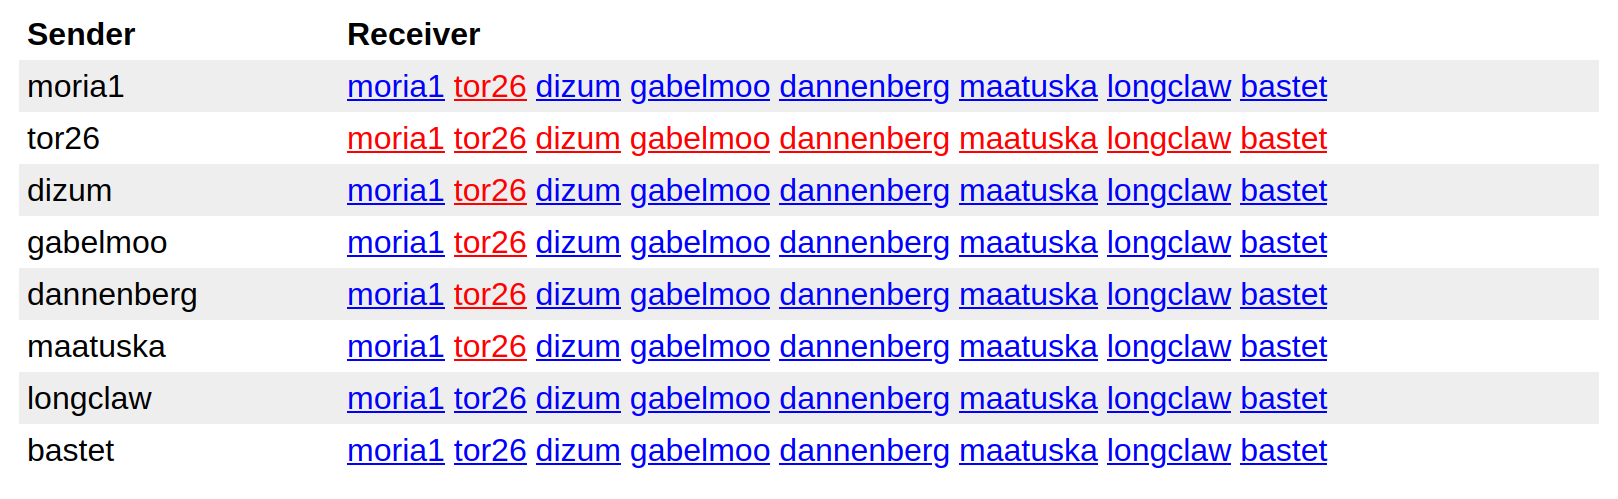
\includegraphics[width=.8\linewidth]{fig/040-remedy.png}\par}
                \end{figure}
                \textbf{Already online and working!}
            \item Patch the protocol so that it is a robust consensus protocol
                \begin{figure}
                    {\centering\includesvg[width=.8\linewidth]{fig/040-dircast.svg}}
                    \caption{Inspired by the famous Dolev-Strong protocol, we design a protocol that secures the directory protocol.}
                \end{figure}
                \begin{figure}
                    {\centering\includesvg[width=.8\linewidth]{fig/050-performance.svg}}
                \end{figure}
                \textbf{Comparable performance with the original protocol!}
        \end{itemize}
    \end{block}
    \begin{block}{\large Check out our paper!}
        \begin{figure}
            {\centering\includesvg[width=.8\linewidth]{fig/qrcode.svg}}
        \end{figure}
    \end{block}
    \end{column}
    \end{columns}
    \vfill
\end{frame}
\end{document}